\def\lecturenumber{09}
\documentclass[11pt,a4paper]{article}
\usepackage[T1]{fontenc}
\usepackage[utf8]{inputenc}
\usepackage{lmodern}
\usepackage[margin=19mm,top=21mm,bottom=21mm,headheight=15pt]{geometry}
\usepackage{amsmath,amssymb,booktabs,array,graphicx,microtype}
\usepackage[dvipsnames]{xcolor}
\usepackage{enumitem,fancyhdr,listings,tcolorbox}
\usepackage[colorlinks=true,linkcolor=MidnightBlue,urlcolor=MidnightBlue]{hyperref}
\definecolor{courseblue}{HTML}{164B69}
\definecolor{pale}{HTML}{F0F5F7}
\pagestyle{fancy}
\fancyhf{}
\fancyhead[L]{\small\sffamily\color{courseblue}VALIDATED COMPUTING}
\fancyhead[R]{\small\sffamily Lecture \lecturenumber}
\fancyfoot[L]{\footnotesize Expanded lecture notes \textbullet\ October 2026}
\fancyfoot[R]{\footnotesize\thepage\ / 6}
\renewcommand{\headrulewidth}{0.4pt}
\setlength{\parindent}{0pt}
\setlength{\parskip}{5.5pt plus 1pt}
\setlength{\emergencystretch}{1.5em}
\setlist[itemize]{leftmargin=1.5em,itemsep=3pt,topsep=3pt}
\setlist[enumerate]{leftmargin=1.7em,itemsep=5pt,topsep=4pt}
\lstset{language=Python,basicstyle=\small\ttfamily,keywordstyle=\color{courseblue}\bfseries,
 commentstyle=\color{OliveGreen},stringstyle=\color{BrickRed},showstringspaces=false,
 columns=fullflexible,keepspaces=true,frame=single,rulecolor=\color{black!18},
 backgroundcolor=\color{black!2},aboveskip=6pt,belowskip=6pt,breaklines=true,
 xleftmargin=5pt,xrightmargin=5pt,framesep=5pt}
\newcommand{\R}{\mathbb R}
\newcommand{\fl}{\operatorname{fl}}
\newcommand{\abs}[1]{\left|#1\right|}
\newcommand{\heading}[2]{\section*{\color{courseblue}#1}\vspace{-4pt}{\small\sffamily\color{black!65}#2}\par\vspace{3pt}}
\newcommand{\opening}[2]{{\Large\sffamily\bfseries\color{courseblue}Lecture \lecturenumber\quad #1\par}\vspace{5pt}{\small #2}\par}
\newtcolorbox{question}[1]{colback=pale,colframe=courseblue!55,boxrule=0.4pt,
 arc=1mm,left=7pt,right=7pt,top=4pt,bottom=4pt,title={#1},fonttitle=\bfseries\small,
 coltitle=courseblue,colbacktitle=pale}
\newcommand{\reading}[1]{{\footnotesize\textbf{Reading and notebook.} #1\par}}
\hypersetup{pdfauthor={Validated Computing course},pdfsubject={Expanded introductory lecture notes with questions and exercises}}

\hypersetup{pdftitle={Lecture 09: Validated roots and complete searches}}
\begin{document}
\opening{Validated roots and complete searches}{Prerequisites: continuity, the mean value theorem, and Lectures 04--08.\newline
Goal: distinguish root claims, derive scalar interval Newton, and preserve every possible root during a search.}
\heading{1. What exactly does a root computation establish?}{0--14 minutes: four claims with different proofs}
An ordinary Newton iteration for $f(x)=x^2-2$ quickly produces a number
close to $1.414213562\ldots$. That is a useful approximation, but a small
residual alone does not prove that a root exists nearby. For instance,
$g(x)=10^{-12}(x-100)$ has residual $10^{-10}$ in magnitude at zero,
although its root is 100 units away. The scale and slope matter.

Separate four questions before choosing a stopping rule:
\begin{center}
\begin{tabular}{p{0.18\linewidth}p{0.72\linewidth}}
\toprule
Claim & A sufficient justification in this course\\
\midrule
Exclusion & A valid image enclosure $F(X)$ excludes zero.\\[4pt]
Existence & Continuity and certified opposite signs at the two endpoints.\\[4pt]
Uniqueness & A derivative enclosure excludes zero, giving at most one root;
combine with a separate existence proof.\\[4pt]
Completeness & A search accounts for every root in the original domain,
with no unresolved regions, and distinguishes the certified roots.\\
\bottomrule
\end{tabular}
\end{center}

For $f(x)=x^2-2$ on $[1,2]$, exact endpoint values are $-1$ and $2$.
Continuity gives a root. The derivative satisfies $f'([1,2])\subseteq[2,4]$,
so $f$ is strictly increasing and has at most one root there. Together these
prove exactly one root in $[1,2]$. They make no claim about the negative
root outside that interval.

The condition $0\in F(X)$ is only failure of an exclusion test. For
$x^2+1$ on $[-1,1]$, an independent-product extension gives $[0,2]$,
yet there is no real root. Similarly, a derivative excluding zero alone
does not establish existence: $x+2$ on $[0,1]$ is strictly increasing
but never zero. Keeping the conclusions separate prevents both mistakes.

\begin{question}{Improve a vague numerical report}
Rewrite ``Newton converged, so the root is correct'' as a precise question
about a specified interval. Which statements are needed to certify exactly
one root there? What additional information would justify ``all roots''?
\end{question}

If a root $r$ is already known to lie in $X$ and $|f'(x)|\ge s>0$ on $X$,
the mean value theorem gives $|t-r|\le |f(t)|/s$ for $t\in X$.
This converts a rigorously bounded residual into an error bound under stated
premises. It is not an existence theorem. Interval Newton will instead
produce a set that every possible root in $X$ must belong to.

\newpage
\heading{2. Derive interval Newton as a root-retention rule}{14--31 minutes: a conditional statement with useful consequences}
Let $f$ be continuously differentiable on a neighborhood of $X=[a,b]$.
Choose $m\in X$, let $C$ enclose $f(m)$, and let the bounded interval $D$
enclose every derivative value on $X$. Assume $0\notin D$. Define
\[
                         N(X)=[m,m]-C/D.
\]
If $r\in X$ is a root distinct from $m$, the mean value theorem gives
\[
 0=f(m)+f'(\xi)(r-m),\qquad
 r=m-\frac{f(m)}{f'(\xi)}\in N(X).
\]
If $r=m$, then $f(m)=0\in C$ and the same inclusion follows directly.
Therefore every root in $X$ lies in $X\cap N(X)$. The argument begins
with ``if a root exists''; it does not assume one into existence.

Two consequences require no further theorem. If $X\cap N(X)$ is empty,
then $X$ contains no root. If the intersection is smaller than $X$, we may
retain it and discard the rest when searching for roots. Those discarded
points may have ordinary function values; they simply cannot be roots.

\textbf{Exact worked step.} For $x^2-2$ on $[1,2]$, choose $m=3/2$.
Then $C=[1/4,1/4]$ and $D=[2,4]$, so
\[
 N(X)=\frac32-\frac{[1/4,1/4]}{[2,4]}
     =\frac32-[1/16,1/8]=[11/8,23/16].
\]
The unique positive root is retained in an interval of width $1/16$.
Its exact midpoint $45/32$ consequently has absolute root error at most
$1/32$. A decimal display of that midpoint is a separate approximation.

\begin{center}
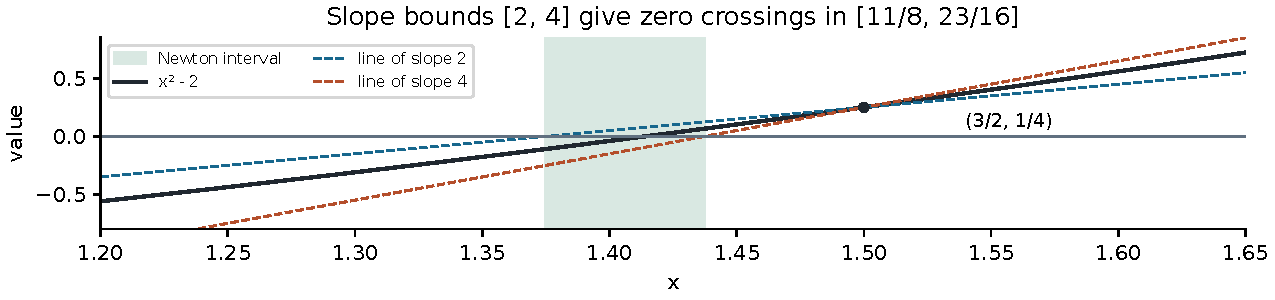
\includegraphics[width=0.88\linewidth]{figures/interval_newton.pdf}
\end{center}

The lines in the figure pass through $(m,f(m))$ with permitted slopes.
Their zero crossings bound possible root locations. The mean value theorem
uses a secant slope to an unknown root; it does not say the derivative at
$m$ alone controls that root. The diagram illustrates the exact calculation.

\begin{question}{A contraction is not yet an existence proof}
If $X\cap N(X)$ is nonempty, what has been established so far? Why must
division be rejected when $D$ contains zero, even if its midpoint is nonzero?
State what may be removed from the search after a valid contraction.
\end{question}

\newpage
\heading{3. Strict inclusion proves existence and uniqueness}{31--48 minutes: prove the scalar theorem and check exact endpoints}
Under the preceding smoothness, enclosure, and nonzero-derivative hypotheses,
a sufficient success test is
\[
                         N(X)\subset\operatorname{int}(X),
 \qquad a<\inf N(X)\ \hbox{and}\ \sup N(X)<b.
\]
This proves that $X$ contains exactly one root, and the root belongs to
$X\cap N(X)$. We use strict interior inclusion deliberately; failure of this
test leaves open cases that another theorem or exact endpoint check may settle.

\textbf{Proof of existence.} First suppose $D$ is positive and write
$c=f(m)\in C$. For any allowed slope $d\in D$, the line
$c+d(t-m)$ crosses zero at $z_d=m-c/d\in N(X)\subset(a,b)$.
It is negative at $a$ and positive at $b$. Apply the mean value theorem
between $m$ and each endpoint: the actual values $f(a)$ and $f(b)$ equal
the corresponding line values for some allowed slopes. Thus
$f(a)<0<f(b)$, and continuity supplies a root. If $m$ is an endpoint,
its value is the line value there for every $d$, so the same argument applies.
For negative $D$, the signs reverse. Finally, $0\notin D$ proves strict
monotonicity and hence uniqueness.

An enclosure $C$ wider than a singleton does not break the proof: it
contains the actual $c$, whose line crossings are among those enclosed by
$N(X)$. Widening may make the success test fail, but cannot manufacture
a false success when all operations preserve inclusion.

Here is a specialized exact-rational step for $x^2-2$ on a positive interval.
It uses no course package and exposes the quotient endpoint order.
\begin{lstlisting}
from fractions import Fraction

def newton_sqrt_two(a, b):
    # Fraction endpoints; the positive domain excludes zero slopes.
    if not 0 < a <= b:
        raise ValueError("Need a positive ordered interval")
    center = (a + b) / 2
    value = center*center - 2
    slope_lower, slope_upper = 2*a, 2*b
    quotients = [value/slope_lower, value/slope_upper]
    return center - max(quotients), center - min(quotients)

a, b = Fraction(1), Fraction(2)
lower, upper = newton_sqrt_two(a, b)
assert (lower, upper) == (Fraction(11, 8), Fraction(23, 16))
assert a < lower and upper < b
assert lower*lower < 2 < upper*upper
\end{lstlisting}

\begin{question}{Two independent ways to read the last lines}
Which assertion checks strict Newton inclusion? Which checks opposite
function signs at the retained endpoints? Why do neither floating-point
equality nor a small printed residual appear in this certificate?
\end{question}

\newpage
\heading{4. Certification and requested accuracy are separate}{48--62 minutes: local decisions and safe refinement}
The first successful Newton test certifies a root even if its enclosure is
wider than a requested plotting or reporting tolerance. After existence and
uniqueness are established, repeated valid intersections refine the same
root without needing a new existence argument on every iteration.

Continue the exact-rational example, starting again at $[1,2]$:
\begin{lstlisting}
a, b = Fraction(1), Fraction(2)
for step in range(4):
    lower, upper = newton_sqrt_two(a, b)
    a = max(a, lower)
    b = min(b, upper)
    if a > b:
        raise ValueError("Contradicts the established root certificate")

assert b - a < Fraction(1, 10**15)
estimate = (a + b) / 2
error_bound = (b - a) / 2
assert error_bound < Fraction(1, 2 * 10**15)
\end{lstlisting}

Here \texttt{estimate} and \texttt{error\_bound} are exact fractions.
The error claim is $|\sqrt2-\texttt{estimate}|\le\texttt{error\_bound}$.
If a decimal approximation $q$ is published instead, account for its
conversion error too: $|\sqrt2-q|\le\texttt{error\_bound}
+|\texttt{estimate}-q|$. Printing fewer digits must not silently preserve
an error bound that referred to a different centre.

For a general interval $X$, a local search decision follows this order:
\begin{enumerate}
\item Evaluate a valid $F(X)$. If it excludes zero, record exclusion.
\item Bound $f'(X)$ by $D$. If $D$ contains zero, this Newton formula is
unavailable; request subdivision rather than division.
\item Compute $N(X)$ and $R=X\cap N(X)$. Empty $R$ proves exclusion.
\item Strict interior inclusion of $N(X)$ certifies exactly one root.
Otherwise, retain a useful contraction $R$, or subdivide $X$.
\end{enumerate}

An interval becoming small is not another certification theorem. In the
course search, the tolerance stops refinement of \emph{undecided} boxes:
they are returned as unresolved. It does not prescribe the width of boxes
that have already passed the root theorem. A separate refinement request,
as above, supplies a numerical error target for a certified root.

\begin{question}{Read a status without adding a claim}
A box has width $10^{-12}$, its image contains zero, and its derivative
image contains zero. How many roots have been proved to lie there? What
should the program report if it cannot afford another subdivision?
\end{question}

The fixed four-step loop here is a checked demonstration for one polynomial.
It is not a promise that four Newton steps attain this accuracy for other
functions. A reusable refiner needs a width check, a budget, and a truthful
status when arithmetic or geometry prevents further improvement.

\newpage
\heading{5. An all-roots claim needs an account of every region}{62--77 minutes: the search invariant and an audit exercise}
Let the original domain be $X_0$. Maintain three collections: pending boxes,
certified root enclosures, and unresolved boxes. Initially $X_0$ is pending.
The essential invariant is
\[
 \{r\in X_0:f(r)=0\}\ \subseteq
 \bigcup\{\text{pending, certified, and unresolved intervals}\}.
\]
Every local action must preserve this statement:
\begin{center}
\begin{tabular}{p{0.18\linewidth}p{0.72\linewidth}}
\toprule
Action & Why no root is lost\\
\midrule
Exclude & A range test or an empty Newton intersection proves no root.\\[4pt]
Certify & The theorem gives one root; retain its certified enclosure.\\[4pt]
Contract & Every root in the old box belongs to its Newton intersection.\\[4pt]
Split & Both closed children together cover the parent.\\[4pt]
Stop & Move every unprocessed box into the unresolved collection.\\
\bottomrule
\end{tabular}
\end{center}

Induction over the decisions proves the invariant for the entire run. A
decision record should preserve the original box, its image, the derivative
bound when used, and the Newton and retained intervals. Otherwise a missing
region may be impossible to distinguish from a justified exclusion.

Unlike a range-cover calculation, a root search may remove non-root points
by contraction. The retained boxes need not cover the original domain as a
set. They must cover its root set, and every removal needs an exclusion or
root-retention argument. Confusing these two invariants leads either to
unnecessary work or to unjustified omissions.

Notebook 09 searches for roots of
\[
                   p(x)=(x+2)(x-1)(x-3),\qquad X_0=[-3,4].
\]
The exact factorization gives reference roots $-2$, $1$, and $3$. The
computational all-roots argument uses local certificates, separation of the
retained root enclosures, and an empty unresolved collection. The known
roots supply an independent diagnostic rather than replacing the search audit.

To conclude that a completed run found exactly $k$ distinct roots, each
reported enclosure must have an existence and uniqueness certificate, the
root enclosures must distinguish $k$ roots (disjointness is a sufficient
check), and the invariant must leave no other possible root unaccounted for.
Overlapping enclosures cannot simply be counted as different roots.

\begin{question}{Audit one decision of each kind}
In the notebook's cubic search, choose a contraction and identify the reason
every removed point is non-root. Choose a split and check both children.
If the budget ends with pending boxes, locate their unresolved records.
What accurate report can replace ``all roots found'' when some remain?
\end{question}

\newpage
\heading{6. Failure cases, exercises, and precise reports}{77--90 minutes: work two examples and write an honest conclusion}
For $x^2$ near zero, the derivative interval includes zero and the taught
Newton division is unavailable. Moreover, there is no sign change across
this double root. For $f(x)=x$ on $[0,1]$, $N(X)=\{0\}$ touches the
boundary, so strict interior inclusion fails. Exact substitution proves the
boundary root, but the course search deliberately has no separate rule for
certifying it. Inconclusive output reflects the chosen tests, not necessarily
a lack of a mathematical answer.

\begin{enumerate}
\item \textbf{Four conclusions.} On $[0,1]$, consider $x+2$ and $x-1/2$.
Use function images, endpoint signs, and derivative bounds to state exactly
what each test establishes. Construct a zero-containing enclosure for a
function that has no root, and explain why inclusion is not the error.

\item \textbf{An exclusion by interval Newton.} Let $f(x)=x^2+1$ on
$X=[1,2]$, with $m=3/2$. Compute $C$, $D$, $N(X)$, and its intersection
with $X$. Which test would already exclude this interval before Newton?
Explain why a general implementation uses that simpler test first.

\item \textbf{A boundary is not an interior.} Compute $N([0,1])$ for
$f(x)=x$. Explain why root retention works while the strict certification
test fails. If both children of a split share an exact root at their common
endpoint, what extra bookkeeping would be needed to count it once?

\item \textbf{Report a partial search.} A run produces two disjoint
certified root enclosures and three unresolved intervals. Write the strongest
conclusion justified by the invariant. Can the unresolved intervals contain
zero, one, or several additional roots? Which records would justify a later
claim of completeness?

\item \textbf{Publish an error bound.} From the first $\sqrt2$ enclosure
$[11/8,23/16]$, compute an exact midpoint and radius. If the midpoint is
replaced by the exact decimal $1.41$, find a safe error bound using the
triangle inequality. Compare it with the bound obtained directly from the
two interval endpoints.
\end{enumerate}

\textbf{Selected checks.} Exercise 1: $x+2$ has no root on the domain;
$x-1/2$ has exactly one. Exercise 2: $C=[13/4,13/4]$, $D=[2,4]$,
$N(X)=[-1/8,11/16]$, so the intersection is empty; $F(X)=[2,5]$ already
excludes zero. Exercise 3: $N(X)=\{0\}$. Exercise 4: at least two distinct
roots exist; every other root in the original domain lies in the unresolved
union. There is no general count for that union. Exercise 5: midpoint
$45/32$, radius $1/32$; the midpoint shift is $3/800$, giving
$1/32+3/800=7/200$. Direct endpoint distances also give $7/200$.

\begin{question}{Exit ticket: a certificate has a scope}
State the function, domain, smoothness and enclosure premises, local success
test, and unresolved status behind one root claim. Explain why a rigorous
certificate for the positive root of $x^2-2$ does not certify all real roots.
\end{question}

\reading{Companion: \texttt{notebooks/09\_validated\_roots.ipynb} and Lab 09.
Tucker (2011), \S\S5.1.1--5.1.3, pp.~73--81, especially Theorem 5.5.
The proof here uses a $C^1$ scalar formulation and a strict success test.
Extended division and scalar Krawczyk methods are optional further reading.}
\end{document}
